\documentclass[11pt,]{article}
\usepackage{lmodern}
\usepackage{amssymb,amsmath}
\usepackage{ifxetex,ifluatex}
\usepackage{fixltx2e} % provides \textsubscript
\ifnum 0\ifxetex 1\fi\ifluatex 1\fi=0 % if pdftex
  \usepackage[T1]{fontenc}
  \usepackage[utf8]{inputenc}
\else % if luatex or xelatex
  \ifxetex
    \usepackage{mathspec}
  \else
    \usepackage{fontspec}
  \fi
  \defaultfontfeatures{Ligatures=TeX,Scale=MatchLowercase}
\fi
% use upquote if available, for straight quotes in verbatim environments
\IfFileExists{upquote.sty}{\usepackage{upquote}}{}
% use microtype if available
\IfFileExists{microtype.sty}{%
\usepackage{microtype}
\UseMicrotypeSet[protrusion]{basicmath} % disable protrusion for tt fonts
}{}
\usepackage[margin = 1.5in]{geometry}
\usepackage{hyperref}
\PassOptionsToPackage{usenames,dvipsnames}{color} % color is loaded by hyperref
\hypersetup{unicode=true,
            pdftitle={Optimization: Part 2},
            pdfauthor={Abhinav Anand, IIMB},
            colorlinks=true,
            linkcolor=blue,
            citecolor=magenta,
            urlcolor=red,
            breaklinks=true}
\urlstyle{same}  % don't use monospace font for urls
\usepackage{color}
\usepackage{fancyvrb}
\newcommand{\VerbBar}{|}
\newcommand{\VERB}{\Verb[commandchars=\\\{\}]}
\DefineVerbatimEnvironment{Highlighting}{Verbatim}{commandchars=\\\{\}}
% Add ',fontsize=\small' for more characters per line
\usepackage{framed}
\definecolor{shadecolor}{RGB}{248,248,248}
\newenvironment{Shaded}{\begin{snugshade}}{\end{snugshade}}
\newcommand{\KeywordTok}[1]{\textcolor[rgb]{0.13,0.29,0.53}{\textbf{#1}}}
\newcommand{\DataTypeTok}[1]{\textcolor[rgb]{0.13,0.29,0.53}{#1}}
\newcommand{\DecValTok}[1]{\textcolor[rgb]{0.00,0.00,0.81}{#1}}
\newcommand{\BaseNTok}[1]{\textcolor[rgb]{0.00,0.00,0.81}{#1}}
\newcommand{\FloatTok}[1]{\textcolor[rgb]{0.00,0.00,0.81}{#1}}
\newcommand{\ConstantTok}[1]{\textcolor[rgb]{0.00,0.00,0.00}{#1}}
\newcommand{\CharTok}[1]{\textcolor[rgb]{0.31,0.60,0.02}{#1}}
\newcommand{\SpecialCharTok}[1]{\textcolor[rgb]{0.00,0.00,0.00}{#1}}
\newcommand{\StringTok}[1]{\textcolor[rgb]{0.31,0.60,0.02}{#1}}
\newcommand{\VerbatimStringTok}[1]{\textcolor[rgb]{0.31,0.60,0.02}{#1}}
\newcommand{\SpecialStringTok}[1]{\textcolor[rgb]{0.31,0.60,0.02}{#1}}
\newcommand{\ImportTok}[1]{#1}
\newcommand{\CommentTok}[1]{\textcolor[rgb]{0.56,0.35,0.01}{\textit{#1}}}
\newcommand{\DocumentationTok}[1]{\textcolor[rgb]{0.56,0.35,0.01}{\textbf{\textit{#1}}}}
\newcommand{\AnnotationTok}[1]{\textcolor[rgb]{0.56,0.35,0.01}{\textbf{\textit{#1}}}}
\newcommand{\CommentVarTok}[1]{\textcolor[rgb]{0.56,0.35,0.01}{\textbf{\textit{#1}}}}
\newcommand{\OtherTok}[1]{\textcolor[rgb]{0.56,0.35,0.01}{#1}}
\newcommand{\FunctionTok}[1]{\textcolor[rgb]{0.00,0.00,0.00}{#1}}
\newcommand{\VariableTok}[1]{\textcolor[rgb]{0.00,0.00,0.00}{#1}}
\newcommand{\ControlFlowTok}[1]{\textcolor[rgb]{0.13,0.29,0.53}{\textbf{#1}}}
\newcommand{\OperatorTok}[1]{\textcolor[rgb]{0.81,0.36,0.00}{\textbf{#1}}}
\newcommand{\BuiltInTok}[1]{#1}
\newcommand{\ExtensionTok}[1]{#1}
\newcommand{\PreprocessorTok}[1]{\textcolor[rgb]{0.56,0.35,0.01}{\textit{#1}}}
\newcommand{\AttributeTok}[1]{\textcolor[rgb]{0.77,0.63,0.00}{#1}}
\newcommand{\RegionMarkerTok}[1]{#1}
\newcommand{\InformationTok}[1]{\textcolor[rgb]{0.56,0.35,0.01}{\textbf{\textit{#1}}}}
\newcommand{\WarningTok}[1]{\textcolor[rgb]{0.56,0.35,0.01}{\textbf{\textit{#1}}}}
\newcommand{\AlertTok}[1]{\textcolor[rgb]{0.94,0.16,0.16}{#1}}
\newcommand{\ErrorTok}[1]{\textcolor[rgb]{0.64,0.00,0.00}{\textbf{#1}}}
\newcommand{\NormalTok}[1]{#1}
\usepackage{graphicx,grffile}
\makeatletter
\def\maxwidth{\ifdim\Gin@nat@width>\linewidth\linewidth\else\Gin@nat@width\fi}
\def\maxheight{\ifdim\Gin@nat@height>\textheight\textheight\else\Gin@nat@height\fi}
\makeatother
% Scale images if necessary, so that they will not overflow the page
% margins by default, and it is still possible to overwrite the defaults
% using explicit options in \includegraphics[width, height, ...]{}
\setkeys{Gin}{width=\maxwidth,height=\maxheight,keepaspectratio}
\IfFileExists{parskip.sty}{%
\usepackage{parskip}
}{% else
\setlength{\parindent}{0pt}
\setlength{\parskip}{6pt plus 2pt minus 1pt}
}
\setlength{\emergencystretch}{3em}  % prevent overfull lines
\providecommand{\tightlist}{%
  \setlength{\itemsep}{0pt}\setlength{\parskip}{0pt}}
\setcounter{secnumdepth}{0}
% Redefines (sub)paragraphs to behave more like sections
\ifx\paragraph\undefined\else
\let\oldparagraph\paragraph
\renewcommand{\paragraph}[1]{\oldparagraph{#1}\mbox{}}
\fi
\ifx\subparagraph\undefined\else
\let\oldsubparagraph\subparagraph
\renewcommand{\subparagraph}[1]{\oldsubparagraph{#1}\mbox{}}
\fi

%%% Use protect on footnotes to avoid problems with footnotes in titles
\let\rmarkdownfootnote\footnote%
\def\footnote{\protect\rmarkdownfootnote}

%%% Change title format to be more compact
\usepackage{titling}

% Create subtitle command for use in maketitle
\newcommand{\subtitle}[1]{
  \posttitle{
    \begin{center}\large#1\end{center}
    }
}

\setlength{\droptitle}{-2em}
  \title{Optimization: Part 2}
  \pretitle{\vspace{\droptitle}\centering\huge}
  \posttitle{\par}
  \author{Abhinav Anand, IIMB}
  \preauthor{\centering\large\emph}
  \postauthor{\par}
  \predate{\centering\large\emph}
  \postdate{\par}
  \date{2018/06/13}

\linespread{1.25}
\usepackage{amsmath}

\begin{document}
\maketitle

\section{Background}\label{background}

The problems seeking to maximize profits or minimize costs often feature
nontrivial constraints which the optimal needs to satisfy. The solution
must lie at the intersection of constraints (for equality constraints)
or on one side of the constraint surface (for inequality constrints).

The problem in a general form is:

\[
\max f(x): x\in \mathbb{R}^n, x\geq 0
\] \[
g_1(x_1,\hdots,x_n)\leq b_1,\hdots,g_k(x_1,\hdots,x_n)\leq b_k
\] \[
h_1(x_1,\hdots,x_n)= c_1,\hdots,h_m(x_1,\hdots,x_n)= c_m
\]

The objective function \(f\) is real valued, i.e.,
\(f:\mathbb{R}^n \to \mathbb{R}\); \(g(\cdot)\) are functional forms of
the \emph{inequality} constraints while \(h(\cdot)\) are functional
forms for the equality constraints.

\section{Equality Constraints}\label{equality-constraints}

Consider the case when \(x=(x_1, x_2)\) and there is a single equality
constraint \(h_1(x) = c_1\).

\[
\max f(x): x\in \mathbb{R}^2, x\geq 0
\] \[
h_1(x) = c_1
\]

To make the illustration more concrete, consider \(f(x) = x_1x_2\) and
\(h_1(x)=c_1:x_1+ x_2=5\).

\begin{Shaded}
\begin{Highlighting}[]
\NormalTok{x_}\DecValTok{1}\NormalTok{ <-}\StringTok{ }\KeywordTok{seq}\NormalTok{(}\FloatTok{0.1}\NormalTok{, }\DecValTok{10}\NormalTok{, }\FloatTok{0.1}\NormalTok{)}
\NormalTok{x_}\DecValTok{2}\NormalTok{ <-}\StringTok{ }\KeywordTok{seq}\NormalTok{(}\FloatTok{0.1}\NormalTok{, }\DecValTok{10}\NormalTok{, }\FloatTok{0.1}\NormalTok{)}

\NormalTok{const_}\DecValTok{1}\NormalTok{ <-}\StringTok{ }\DecValTok{1}
\NormalTok{const_}\DecValTok{2}\NormalTok{ <-}\StringTok{ }\DecValTok{2}
\NormalTok{const_}\DecValTok{3}\NormalTok{ <-}\StringTok{ }\DecValTok{3}

\NormalTok{f_x_level_}\DecValTok{1}\NormalTok{ <-}\StringTok{ }\NormalTok{const_}\DecValTok{1}\OperatorTok{/}\NormalTok{x_}\DecValTok{2} \CommentTok{#level sets}
\NormalTok{f_x_level_}\DecValTok{2}\NormalTok{ <-}\StringTok{ }\NormalTok{const_}\DecValTok{2}\OperatorTok{/}\NormalTok{x_}\DecValTok{2}
\NormalTok{f_x_level_}\DecValTok{3}\NormalTok{ <-}\StringTok{ }\NormalTok{const_}\DecValTok{3}\OperatorTok{/}\NormalTok{x_}\DecValTok{2}

\NormalTok{x_}\DecValTok{3}\NormalTok{ <-}\StringTok{ }\DecValTok{5} \OperatorTok{-}\StringTok{ }\NormalTok{x_}\DecValTok{2} \CommentTok{#constraint set}

\NormalTok{data_obj_l <-}\StringTok{ }\KeywordTok{cbind}\NormalTok{(x_}\DecValTok{1}\NormalTok{, }
\NormalTok{                    f_x_level_}\DecValTok{1}\NormalTok{, }
\NormalTok{                    f_x_level_}\DecValTok{2}\NormalTok{, }
\NormalTok{                    f_x_level_}\DecValTok{3}\NormalTok{,}
\NormalTok{                    x_}\DecValTok{3}
\NormalTok{                    ) }\OperatorTok\StringTok{ }
\StringTok{  }\NormalTok{dplyr}\OperatorTok{::}\KeywordTok{as_tibble}\NormalTok{() }\OperatorTok
\StringTok{  }\NormalTok{tidyr}\OperatorTok{::}\KeywordTok{gather}\NormalTok{(.,}
\NormalTok{                f_x_level_}\DecValTok{1}\OperatorTok{:}\NormalTok{x_}\DecValTok{3}\NormalTok{,}
                \DataTypeTok{key =} \StringTok{"f"}\NormalTok{,}
                \DataTypeTok{value =} \StringTok{"levels"}\NormalTok{)}


\KeywordTok{ggplot}\NormalTok{(data_obj_l, }\KeywordTok{aes}\NormalTok{(x_}\DecValTok{1}\NormalTok{, levels, }\DataTypeTok{color =}\NormalTok{ f)) }\OperatorTok{+}
\StringTok{  }\KeywordTok{geom_line}\NormalTok{() }\OperatorTok{+}
\StringTok{  }\KeywordTok{scale_y_continuous}\NormalTok{(}\DataTypeTok{limits =} \KeywordTok{c}\NormalTok{(}\DecValTok{0}\NormalTok{, }\DecValTok{10}\NormalTok{)) }\OperatorTok{+}
\StringTok{  }\KeywordTok{scale_x_continuous}\NormalTok{(}\DataTypeTok{limits =} \KeywordTok{c}\NormalTok{(}\DecValTok{0}\NormalTok{, }\DecValTok{10}\NormalTok{)) }\OperatorTok{+}
\StringTok{  }\KeywordTok{theme_minimal}\NormalTok{()}
\end{Highlighting}
\end{Shaded}

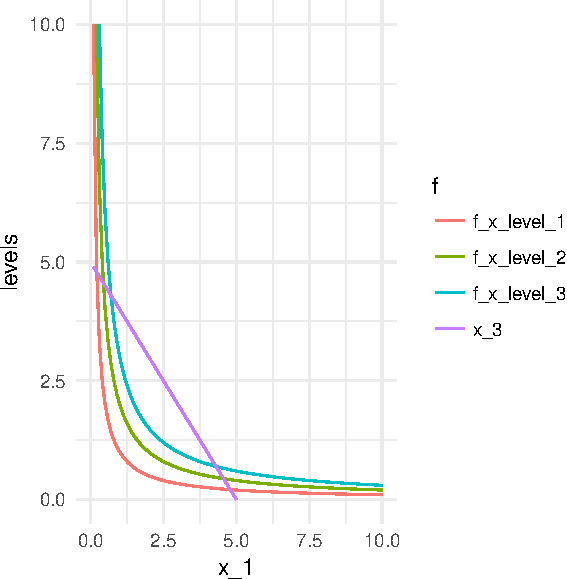
\includegraphics{Optimization_2_files/figure-latex/opt_dim_2-1.pdf}

Geometrically we need to find the highest valued level set for
\(f(x) = x_1x_2\) that satisfies \(x_1+x_2=5, x_1, x_2\geq 0\). The key
observation is the following: at the optimal, the levels sets and the
constraint set must be tangent---just touching (intersecting) each other
at exactly one point. (Why must this be so? What happens if there the
plots cross over? Can we improve the objective function then?)


\end{document}
